To navigate the map, all you need is a regular mouse or touchpad that can scroll.

To zoom in and out, you simply need to point the cursor at the map and scroll. When zooming in, the map will zoom in on the location the cursor is currently pointing at. This means that if there is a certain area on the map that you want to zoom in on, you just need to place the cursor on that area and scroll. When zooming out, the position of the cursor is irrelevant. The more you zoom in, the more roads and details will you be able to see.

If the area you have zoomed in on is not exactly the area you want to view, you can navigate around the map by dragging up, down and to the sides, to find the area you want to view. This is done by left-clicking on the map, holding down the left mouse button while dragging the cursor. \\
\begin{figure}[htb]
\centering
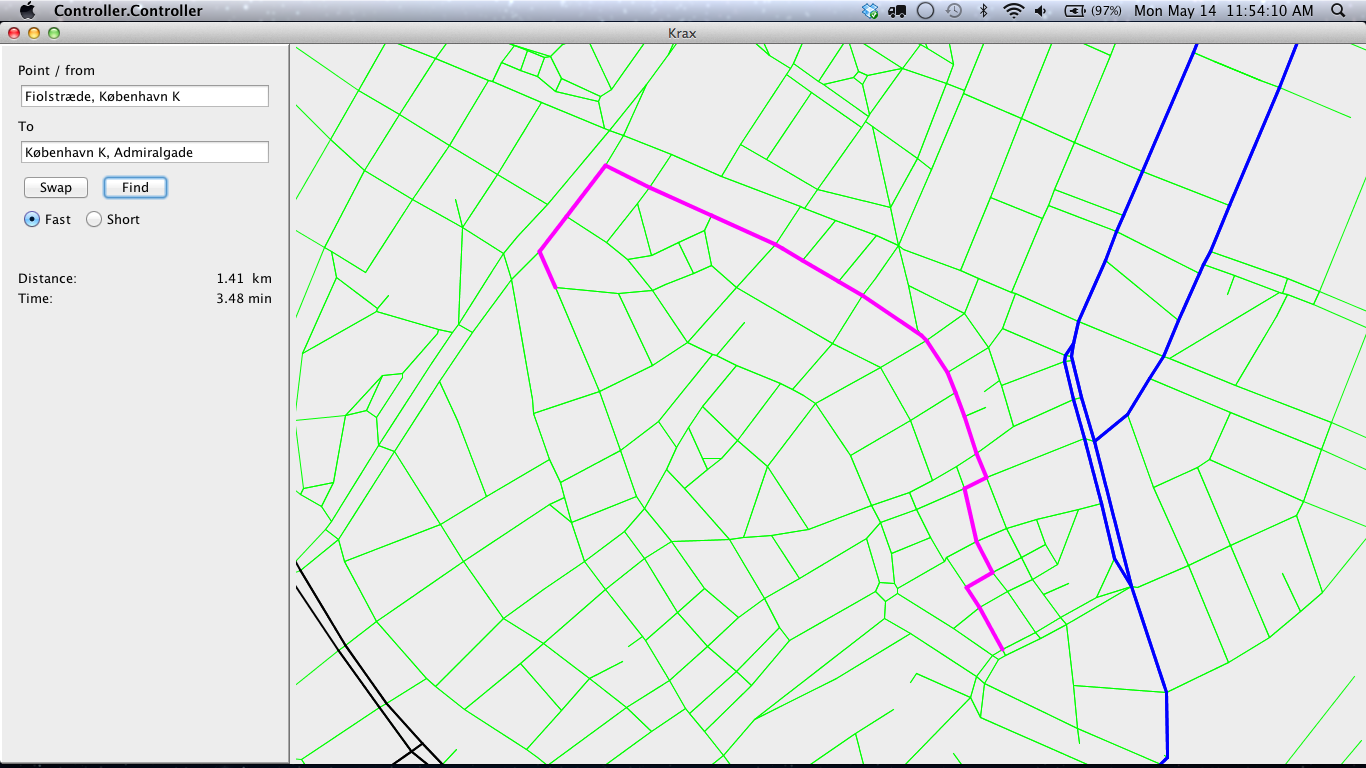
\includegraphics[scale=0.25]{User_manual/screenshot.png}
\end{figure}
